\documentclass{article}

\usepackage[letterpaper,left=2.2cm,right=2.2cm,top=2.2cm,bottom=2.3cm]{geometry}
\usepackage[T1]{fontenc}
\usepackage[spanish,es-nodecimaldot]{babel}
\usepackage{tgheros}
\renewcommand{\familydefault}{\sfdefault}

\usepackage{amsmath}
\usepackage{array}
\usepackage{booktabs}
\usepackage{caption}
\usepackage[americanresistors]{circuitikz}
\usepackage{fancyhdr}
\usepackage{float}
\usepackage{graphicx}
\usepackage{microtype}
\usepackage{subcaption}
\usepackage{tabularx}
\usepackage{xcolor}
\usepackage{siunitx}
\sisetup{
    output-decimal-marker = {,}
}
\usepackage{pgfplots}
\usepackage[hidelinks]{hyperref}

\pgfplotsset{compat=1.18}
\graphicspath{{./}{../}}

\definecolor{utnblue}{HTML}{164B72}
\definecolor{softblue}{HTML}{EAF2F7}
\definecolor{softgray}{HTML}{F3F4F5}
\definecolor{alertred}{HTML}{8A2B2B}

\captionsetup{font=small,labelfont=bf}
\setlength{\parindent}{0pt}
\setlength{\parskip}{0.55em}
\setlength{\tabcolsep}{5pt}
\renewcommand{\arraystretch}{1.15}
\setcounter{tocdepth}{2}

\pagestyle{fancy}
\fancyhf{}
\fancyhead[L]{Electrónica Aplicada II}
\fancyhead[R]{TP1 -- Control de Tonos Baxandall}
\fancyfoot[C]{\thepage}
\renewcommand{\headrulewidth}{0.4pt}

\newcommand{\measurementtable}[1]{%
    \begin{table}[H]
    \centering
    \small
    #1
    \end{table}
}

\newcommand{\minsweepcapture}[2]{%
    \begin{subfigure}[t]{0.45\textwidth}
        \centering
        \includegraphics[width=\linewidth]{freq_sweep_pot_min_#1.jpeg}
        \caption{Medición #1: \(#2\).}
    \end{subfigure}%
}

\newcommand{\maxsweepcapture}[2]{%
    \begin{subfigure}[t]{0.45\textwidth}
        \centering
        \includegraphics[width=\linewidth]{freq_sweep_pot_max_#1.jpeg}
        \caption{Medición #1: \(#2\).}
    \end{subfigure}%
}

\newcommand{\midsweepcapture}[2]{%
    \begin{subfigure}[t]{0.45\textwidth}
        \centering
        \includegraphics[width=\linewidth]{freq_sweep_pot_mid_#1.jpeg}
        \caption{Medición #1: \(#2\).}
    \end{subfigure}%
}

\begin{document}

\pagenumbering{gobble}
\newgeometry{left=61bp,right=61bp,top=0pt,bottom=0pt}

\begin{titlepage}
\thispagestyle{empty}
\setlength{\unitlength}{1bp}
\setlength{\parindent}{0pt}
\fontencoding{T1}\fontfamily{qhv}\selectfont

\centering
\begin{picture}(490,792)(0,0)
    % Main form
    \linethickness{2bp}
    \put(0,132){\framebox(490,600){}}
    \put(0,660){\line(1,0){490}}
    \put(0,614){\line(1,0){490}}
    \put(0,552){\line(1,0){490}}
    \put(0,511){\line(1,0){490}}
    \put(0,463){\line(1,0){490}}
    \put(0,329){\line(1,0){490}}
    \put(0,275){\line(1,0){490}}
    \put(0,234){\line(1,0){490}}
    \put(0,182){\line(1,0){490}}

    % Form title
    \put(0,696){\makebox(490,0)[c]{\fontsize{15}{16}\selectfont\bfseries UNIVERSIDAD TECNOLOGICA NACIONAL}}
    \put(0,680){\makebox(490,0)[c]{\fontsize{15}{16}\selectfont\bfseries FACULTAD REGIONAL AVELLANEDA}}

    % Form contents
    \put(35,622){\makebox(0,0)[l]{\fontsize{12}{14}\selectfont\underline{ASIGNATURA:}}}
    \put(177,622){\makebox(0,0)[l]{\fontsize{12}{14}\selectfont Electrónica Aplicada II}}

    \put(35,567){\makebox(0,0)[l]{\fontsize{12}{14}\selectfont\underline{TRABAJO PRACTICO N\textdegree{}:}}}
    \put(212,567){\makebox(0,0)[l]{\fontsize{12}{14}\selectfont 1 -- Control de Tonos Baxandall}}

    \put(35,526){\makebox(0,0)[l]{\fontsize{12}{14}\selectfont\underline{PROFESOR:} Ing. Sergio Martínez}}
    \put(36,484){\makebox(0,0)[l]{\fontsize{12}{14}\selectfont\underline{AYUDANTE:} Ing. Leonel Fulcheri}}

    \put(35,429){\makebox(0,0)[l]{\fontsize{12}{14}\selectfont\underline{ALUMNOS:}}}
    \put(35,398){\makebox(0,0)[l]{\fontsize{12}{14}\selectfont
            \shortstack{Lahorca Nicolás\\[2pt]Silva Hernán\\[2pt]Justiniano Luciano}%
    }%
}
    \put(283,429){\makebox(0,0)[l]{\fontsize{12}{14}\selectfont\underline{CURSO:} 4\textdegree{}12}}

    \put(35,291){\makebox(0,0)[l]{\fontsize{12}{14}\selectfont\underline{ESPECIALIDAD:}}}
    \put(143,291){\makebox(0,0)[l]{\fontsize{12}{14}\selectfont Ingeniería en Electrónica}}
    \put(319,291){\makebox(0,0)[l]{\fontsize{12}{14}\selectfont\underline{GRUPO:} 2}}

    \put(35,250){\makebox(0,0)[l]{\fontsize{12}{14}\selectfont\underline{FECHA DE REALIZACIÓN:} 13 de septiembre de 2026}}
    \put(35,209){\makebox(0,0)[l]{\fontsize{12}{14}\selectfont\underline{FECHA Y FIRMA DE APROBACIÓN DEL T.P.:}}}
    \put(35,153){\makebox(0,0)[l]{\fontsize{12}{14}\selectfont\underline{FIRMA DEL ALUMNO:}}}
\end{picture}
\end{titlepage}

\restoregeometry


\pagenumbering{arabic}
\tableofcontents
\clearpage

\section*{Introducción}
\addcontentsline{toc}{section}{Introducción}

El presente trabajo estudia un control de tonos Baxandall activo para la banda de audio de
\(20\,\mathrm{Hz}\) a \(20\,\mathrm{kHz}\). El circuito se alimenta desde una fuente simple de
\(15\,\mathrm{V}\); un regulador LM78L12 entrega \(12\,\mathrm{V}\) a la electrónica y dos
amplificadores operacionales RC4558 realizan el acondicionamiento de entrada y el control de
tonos.

Las mediciones se efectuaron con una señal senoidal de aproximadamente \(1\,\mathrm{V_p}\),
de acuerdo con la consigna. En las capturas, CH1 corresponde a la entrada y CH2 a la salida.
Los resultados numéricos del barrido se transcriben sin alterar las denominaciones ni los
valores de las tablas PDF entregadas.

\section{Verificación mediante simulación}

La verificación previa se conserva en el archivo editable \texttt{EQ\_Baxandall\_sim.asc},
que contiene el circuito para análisis de pequeña señal. El objetivo del análisis es comprobar
la continuidad de la respuesta en la banda de audio y observar el efecto de las posiciones de
los controles antes de efectuar las mediciones sobre la placa.

La consigna solicita específicamente una captura de la simulación realizada en TINA. No se
incluye una imagen sustituta porque no existe una captura de TINA entre los archivos provistos.

\section{Diseño y construcción del circuito impreso}

Para la construcción del circuito se utilizó una placa de 10 mm por 5 mm.

\begin{figure}[H]
    \centering
    \includegraphics[page=1,width=\textwidth]{../sch.pdf}
    \caption{Esquema eléctrico implementado en KiCad.}
    \label{fig:schematic}
\end{figure}

\section{Etapas del circuito y adaptación a fuente simple}

El circuito se divide en las siguientes 3 etapas:

\begin{enumerate}
    \item \textbf{Etapa de alimentación} Etapa consituída por el regulador de tensión
        LM7812 (U1), encargado de proveer los 12 V a todo el circuito.

    \item \textbf{Etapa inversora} Su núcleo está compuesto por uno de los dos
        amplificadores operacionales disponibles en el integrado RC4558 (U2B). La función de
        esta etapa es invertir la señal de audio de entrada, ya que la etapa siguiente
        también es inversora.

    \item \textbf{Control Baxandall} La segunda mitad del RC4558 trabaja con una red
    de realimentación selectiva. RV1, RV2, R1, R2, R4, R6 y los capacitores C4, C5, C12 y C13
    modifican la realimentación según la frecuencia, permitiendo realce o atenuación de
    los tonos graves y agudos de la señal de audio de entrada.
\end{enumerate}

La modificación fundamental para que el circuito pueda funcionar con fuente simple es la
creación de la referencia de \(6\,\mathrm{V}\) mediante el divisor resistivo conformado
por R3 y R5. Esto logra centrar la señal en la mitad de la alimentación, lo que  permite
procesar ambos semiciclos sin que los mismos sean recortados.

\section{Excursión de salida y máxima señal de entrada}
El datasheet del operacional RC4558 indica que la tensión de salida del mismo
es aproximadamente $V_{CC} \pm \SI{1}{\volt}$; la alimentación en este caso es
$+\SI{12}{\volt}$ y $\SI{0}{\volt}$, por lo que

\[
\begin{gathered}
    V_{oMax} = \SI{11}{\volt} \\
    V_{oMin} = \SI{1}{\volt}
\end{gathered}
\]

Para lograr alimentar con fuente simple al cricuito, los operacionales
utilizados poseen una referencia de $\SI{6}{\volt}$, por lo tanto solo se puede
excursionar $\pm \SI{5}{\volt}$ para que los semiciclos de la señal no sean
distorsionados.\par
Como se demosatrará en el punto 5, la mayor ganancia del circuito ocurre con
las frecuencias bajas, donde Av es 11,2, por lo tanto el
máximo nivel de señal de entrada se puede calcular como

\[
\begin{gathered}
    V_i = \frac{Vo_{max}}{Av} \\[2pt]
    V_i = \frac{\SI{5}{\volt}p}{11,2} \\[2pt]
    \boxed{V_i = \SI{0{,}446}{\volt}p}
\end{gathered}
\]

\section{Cálculo de ganancias}
El potenciómetro RV1 del esquemático es el encargado de modificar la ganancia de las
frecuencias bajas. Esto es debido a que los capacitores C12 y C13 se comportan como
circuito abierto cuando están sometidos a frecuencias bajas, esto se justifica con la
expresión de la reactancia capacitiva.

\begin{equation}
    X_C = \frac{1}{2\pi f C}
    \label{eq:xcap}
\end{equation}

Si se aplica la misma ecuación pero en frecuencias altas, se puede decir que
los capacitores se comportan como corto circuito en frecuencias elevadas; por
lo que C4 y C5 puentean a RV1 en frecuencias altas. quedando como regulador de
ganancia el potenciómetro RV2.

\subsection{Ganancia en bajas frecuencias}

\begin{figure}[H]
    \centering
    \begin{circuitikz}[font=\small]
        \node[op amp] (U2A) at (6,0) {};

        \draw
            (0,3) node[ocirc] {}
            node[left,align=right]{Entrada\\(desde C9)}
            to[R,l^={$R_1$},a_={$10\,\mathrm{k}\Omega$}] (2,3)
            to[R] (4,3)
            to[R,l^={$R_2$},a_={$12\,\mathrm{k}\Omega$}] (7.2,3)
            -- (8,3) node[ocirc] {}
            node[right]{Salida};

        \draw (7.2,3) to[short,*-] (7.2,0) -- (U2A.out);
        \node[above=7pt,align=center] at (3,3)
            {$RV_1$\\[-1pt]$100\,\mathrm{k}\Omega$};
        \draw (3,2.15) to[R,l={$R_4$},a_={$10\,\mathrm{k}\Omega$}] (3,0.5)
            -- (U2A.-);
        \draw (3,2.15) -- (3,2.72);
        \fill (3,2.85) -- (2.91,2.68) -- (3.09,2.68) -- cycle;

        \draw (U2A.+) -- (3.7,-0.5) node[ocirc] {}
            node[left] {$V_{\mathrm{ref}}\;(\sim 6\,\mathrm{V})$};

        \node[align=center,font=\tiny] at (6.08,0.04) {$U2A$\\[-1.5pt]RC4558};
        \node[above left=1pt] at (U2A.-) {2};
        \node[below left=1pt] at (U2A.+) {3};
        \node[above right=1pt] at (U2A.out) {1};
    \end{circuitikz}
    \caption{Equivalente resistivo del control de bajas frecuencias}
    \label{fig:low-frequency-equivalent}
\end{figure}

De la fig. \ref{fig:low-frequency-equivalent} se puede observar que el circuito
se simplifica a un inversor. Por lo tanto la ganancia se calcula como

\begin{equation*}
    Av = - \frac{R_f}{R}
\end{equation*}

\begin{itemize}
    \item \textbf{RV1 con el cursor al mínimo}
        \[
        \begin{gathered}
            Av = - \frac{R_2}{R_1 + RV_{1}} \\[2pt]
            Av = - \frac{\SI{12}{\kilo\ohm}}{\SI{10}{\kilo\ohm} + \SI{100}{\kilo\ohm}} \\[2pt]
            \boxed{Av = -0,109} \\[2pt]
            \boxed{Av = \SI{-19{,}25}{\decibel}}
        \end{gathered}
        \]
    \item \textbf{RV1 con el cursor al máximo}
        \[
        \begin{gathered}
            Av = - \frac{RV_1 + R_2}{R_1} \\[2pt]
            Av = - \frac{\SI{100}{\kilo\ohm} + \SI{12}{\kilo\ohm}}{\SI{10}{\kilo\ohm}} \\[2pt]
            \boxed{Av = -11,2} \\[2pt]
            \boxed{Av = \SI{20{,}98}{\decibel}}
        \end{gathered}
        \]
\end{itemize}

\subsection{Ganancia en altas frecuencias}

\begin{figure}[H]
    \centering
    \begin{circuitikz}[font=\small]
        \node[op amp] (U2AHF) at (6,0) {};

        \draw
            (0,3) node[ocirc] {}
            node[left,align=right]{Entrada\\(desde C9)}
            -- (0.8,3) coordinate (hfin)
            to[R,l^={$R_1$},a_={$10\,\mathrm{k}\Omega$}] (3.4,3)
            coordinate (hfr4)
            to[R,l^={$R_2$},a_={$12\,\mathrm{k}\Omega$}] (7.2,3)
            coordinate (hfout)
            -- (8,3) node[ocirc] {}
            node[right]{Salida};

        \draw (hfout) to[short,*-] (7.2,0) -- (U2AHF.out);
        \node[circ] at (7.2,0) {};
        \node[above=5pt] at (hfr4) {$A$};
        \draw (hfr4) to[short,*-] (3.4,2.5)
            to[R,l={$R_4$},a_={$10\,\mathrm{k}\Omega$}] (3.4,0.5)
            to[short,*-] (U2AHF.-);

        \draw (3.4,0.5) -- (3.4,-0.8)
            to[R,l={$R_6$},a_={$4{,}7\,\mathrm{k}\Omega$}] (3.4,-2.05)
            -- (3.4,-2.52);

        \draw (hfin) to[short,*-] (0.8,-2.8)
            -- (2.4,-2.8)
            to[R] (4.4,-2.8)
            -- (7.2,-2.8) -- (hfout);
        \node[below=7pt,align=center] at (3.4,-2.8)
            {$RV_2$\\[-1pt]$100\,\mathrm{k}\Omega$};
        \fill (3.4,-2.65) -- (3.31,-2.48) -- (3.49,-2.48) -- cycle;

        \draw (U2AHF.+) -- (2.8,-0.5) node[ocirc] {}
            node[left] {$V_{\mathrm{ref}}\;(\sim 6\,\mathrm{V})$};

        \node[align=center,font=\tiny] at (6.08,0.04)
            {$U2A$\\[-1.5pt]RC4558};
        \node[above left=1pt] at (U2AHF.-) {2};
        \node[below left=1pt] at (U2AHF.+) {3};
        \node[above right=1pt] at (U2AHF.out) {1};
    \end{circuitikz}
    \caption{Equivalente resistivo del control de altas frecuencias}
    \label{fig:high-frequency-equivalent}
\end{figure}

Para analizar este circuito es conveniente aplicar la ley de kirchoff de las
corrientes en el nodo que une el terminal inversor del operacional con las
resistencias R4 y R6. El análisis es sobre la señal de audio, por lo que las
fuentes de corriente continua se pasivan.

\begin{figure}[H]
    \centering
    \begin{circuitikz}[font=\small]
        \node[op amp] (U2ANodal) at (6.2,0) {};
        \coordinate (summing) at (3,0.5);

        \draw (3,3) node[ocirc] {}
            to[R] (summing)
            to[short,*-] (U2ANodal.-);
        \draw (summing)
            to[R] (3,-2)
            node[ocirc] {};
        \node[right=5pt,align=left] at (3,1.75)
            {$R_4$\\[-1pt]$10\,\mathrm{k}\Omega$};
        \node[right=5pt,align=left] at (3,-0.75)
            {$R_6$\\[-1pt]$4{,}7\,\mathrm{k}\Omega$};

        \draw[-latex] (2.45,2.45) -- (2.45,1.15)
            node[midway,left] {$I_{R_4}$};
        \draw[-latex] (2.45,-1.45) -- (2.45,-0.15)
            node[midway,left] {$I_{R_6}$};
        \draw[-latex] (3.4,0.72) -- (4.7,0.72)
            node[midway,above] {$I_i$};

        \draw (U2ANodal.+) -- (4.85,-0.5) -- (4.85,-0.85)
            node[ground] {};
        \draw (U2ANodal.out) -- (7.5,0) node[ocirc] {};

        \draw[-latex,densely dashed,utnblue] (0.65,0.75)
            node[left,align=right,text=utnblue]{TV\\(tierra virtual)}
            -- (2.82,0.55);

        \node[align=center,font=\tiny] at (6.28,0.04)
            {$U2A$\\[-1.5pt]RC4558};
    \end{circuitikz}
    \caption{Corrientes en el nodo de tierra virtual del amplificador operacional}
    \label{fig:high-frequency-current-node}
\end{figure}
 
Por la figura se obtiene

\begin{equation*}
    I_{R_4} + I_{R_6} = I_i = 0
\end{equation*}

\begin{equation}
    I_{R_4} = - I_{R_6}
    \label{eq:vi}
\end{equation}

Además, al aplicar la misma ley en el nodo A de la fig.
\ref{fig:high-frequency-equivalent}

\[
\begin{gathered}
    I_{R_1} + I_{R_2} = I_{R_4} \\[2pt]
    \frac{V_i - V_A}{R_1} + \frac{V_o - V_A}{R_2} = I_{R_4} \\[2pt]
    \frac{V_i}{R1} - \frac{V_A}{R1} + \frac{V_o}{R2} - \frac{V_A}{R_2} = \frac{V_A}{R_4}
\end{gathered}
\]

Despejando $V_A$ se llega a la expresión

\begin{equation}
    V_A = \frac{V_i}{\frac{R1}{R_4} + \frac{R1}{R2} + 1} + \frac{V_o}{\frac{R2}{R_4} + \frac{R2}{R1} + 1} 
    \label{eq:va}
\end{equation}

Teniendo en cuenta la posición del cursor del potenciómetro RV2 y reemplazando
(\ref{eq:va}) en (\ref{eq:vi}) se pueden llegar a los siguientes 2 resultados
%\newpage

\begin{itemize}
    \item \textbf{RV2 con el cursor al mínimo}
        \begin{figure}[H]
            \centering
            \begin{circuitikz}[font=\small]
                \node[op amp] (U2AHFMin) at (6,0) {};

                \draw
                    (0,3) node[ocirc] {}
                    node[left,align=right]{$V_i$}
                    -- (0.8,3) coordinate (hfminin)
                    to[R,l^={$R_1$},a_={$10\,\mathrm{k}\Omega$}] (3.4,3)
                    coordinate (hfmina)
                    to[R,l^={$R_2$},a_={$12\,\mathrm{k}\Omega$}] (7.2,3)
                    coordinate (hfminout)
                    -- (8,3) node[ocirc] {}
                    node[right]{$V_o$};

                \draw (hfminout) to[short,*-] (7.2,0) -- (U2AHFMin.out);
                \node[circ] at (7.2,0) {};
                \node[above=5pt] at (hfmina) {$A$};

                \draw (hfmina) to[short,*-] (3.4,2.5)
                    to[R,l={$R_4$},a_={$10\,\mathrm{k}\Omega$}] (3.4,0.5)
                    to[short,*-] (U2AHFMin.-);
                \draw (3.4,0.5) -- (3.4,-0.8)
                    to[R,l={$R_6$},a_={$4{,}7\,\mathrm{k}\Omega$}] (3.4,-2.3)
                    -- (3.4,-2.8);

                \draw (hfminin) to[short,*-] (0.8,-2.8)
                    -- (1.1,-2.8)
                    to[R,l={$RV_2$},a_={$100\,\mathrm{k}\Omega$}] (3.1,-2.8)
                    -- (3.4,-2.8) coordinate (hfminb)
                    -- (7.2,-2.8) -- (hfminout);
                \node[circ] at (hfminb) {};
                \node[below=5pt] at (hfminb) {$B$};

                \draw (U2AHFMin.+) -- ++(-0.45,0) coordinate (gndMin);
                \draw (gndMin) -- ++(0,-0.45) node[ground] {};

                \node[align=center,font=\tiny] at (6.08,0.04)
                    {$U2A$\\[-1.5pt]RC4558};
                \node[above left=1pt] at (U2AHFMin.-) {2};
                \node[below left=1pt] at (U2AHFMin.+) {3};
                \node[above right=1pt] at (U2AHFMin.out) {1};
            \end{circuitikz}
            \caption{Equivalente resistivo de altas frecuencias con el cursor de RV2
            desplazado completamente hacia la derecha}
            \label{fig:high-frequency-rv2-min}
        \end{figure}

        Se puede ver que el nodo $V_B = V_o$. Entonces

        \[
        \begin{gathered}
            \frac{\frac{V_i}{\frac{R1}{R_4} + \frac{R1}{R2} + 1} + \frac{V_o}{\frac{R2}{R_4} + \frac{R2}{R1} + 1}}{R_4} = -\frac{V_o}{R_6} \\[2pt]
            \frac{V_i}{\frac{R_1 R_4}{R_2} + R_1 + R_4} + \frac{V_o}{\frac{R_2 R_4}{R1} + R_2 + R_4} = -\frac{V_o}{R_6} \\[2pt]
            \frac{Vo}{Vi} = \frac{1}{\left(\frac{R_2 R_4}{R_1} + R_1 + R_4\right)\left(- \frac{1}{\frac{R_2 R_4}{R_1} + R_2 + R_4} - \frac{1}{R_6}\right)} \\[2pt]
            \boxed{Av = -0{,}146} \\[2pt]
            \boxed{Av = \SI{-16{,}71}{\decibel}}
        \end{gathered}
        \]
    \newpage

    \item \textbf{RV2 con el cursor al máximo}

        En este caso sucede algo similar al anterior, con la
        diferencia de que ahora el nodo B está conectado directamente en la
        entrada, es decir, $V_B = V_i$.

        \begin{figure}[H]
            \centering
            \begin{circuitikz}[font=\small]
                \node[op amp] (U2AHFMax) at (6,0) {};

                \draw
                    (0,3) node[ocirc] {}
                    node[left] {$V_i$}
                    -- (0.8,3) coordinate (hfmaxin)
                    to[R,l^={$R_1$},a_={$10\,\mathrm{k}\Omega$}] (3.4,3)
                    coordinate (hfmaxa)
                    to[R,l^={$R_2$},a_={$12\,\mathrm{k}\Omega$}] (7.2,3)
                    coordinate (hfmaxout)
                    -- (8,3) node[ocirc] {}
                    node[right] {$V_o$};

                \draw (hfmaxout) to[short,*-] (7.2,0) -- (U2AHFMax.out);
                \node[circ] at (7.2,0) {};
                \node[above=5pt] at (hfmaxa) {$A$};

                \draw (hfmaxa) to[short,*-] (3.4,2.5)
                    to[R,l={$R_4$},a_={$10\,\mathrm{k}\Omega$}] (3.4,0.5)
                    to[short,*-] (U2AHFMax.-);
                \draw (3.4,0.5) -- (3.4,-0.8)
                    to[R,l={$R_6$},a_={$4{,}7\,\mathrm{k}\Omega$}] (3.4,-2.3)
                    -- (3.4,-2.8) coordinate (hfmaxb);

                \draw (hfmaxin) to[short,*-] (0.8,-2.8)
                    -- (hfmaxb)
                    -- (3.7,-2.8)
                    to[R,l={$RV_2$},a_={$100\,\mathrm{k}\Omega$}] (5.7,-2.8)
                    -- (7.2,-2.8) -- (hfmaxout);
                \node[circ] at (hfmaxb) {};
                \node[below=5pt] at (hfmaxb) {$B$};

                \draw (U2AHFMax.+) -- ++(-0.45,0) coordinate (gndMax);
                \draw (gndMax) -- ++(0,-0.45) node[ground] {};

                \node[align=center,font=\tiny] at (6.08,0.04)
                    {$U2A$\\[-1.5pt]RC4558};
                \node[above left=1pt] at (U2AHFMax.-) {2};
                \node[below left=1pt] at (U2AHFMax.+) {3};
                \node[above right=1pt] at (U2AHFMax.out) {1};
            \end{circuitikz}
            \caption{Equivalente resistivo de altas frecuencias con el cursor de RV2
            desplazado completamente hacia la izquierda}
            \label{fig:high-frequency-rv2-max}
        \end{figure}

        \[
        \begin{gathered}
            \frac{\frac{V_i}{\frac{R1}{R_4} + \frac{R1}{R2} + 1} + \frac{V_o}{\frac{R2}{R_4} + \frac{R2}{R1} + 1}}{R_4} = -\frac{V_i}{R_6} \\[2pt]
            \frac{V_i}{\frac{R_1 R_4}{R_2} + R_1 + R_4} + \frac{V_o}{\frac{R_2 R_4}{R1} + R_2 + R_4} = -\frac{V_i}{R_6} \\[2pt]
            \frac{Vo}{Vi} = \left(-\frac{1}{R_6} - \frac{1}{\frac{R_1 R_4}{R_2} + R_1 + R_4}\right) \left(\frac{R_2 R_4}{R_1} + R_2 + R_4\right) \\[2pt]
            \boxed{Av = -8{,}434} \\[2pt]
            \boxed{Av = \SI{18{,}52}{\decibel}}
        \end{gathered}
        \]
\end{itemize}

\section{Potenciómetros al máximo}

Para los puntos 6 a 9 se calculó la ganancia a partir de las amplitudes pico a pico visibles en
las capturas o consignadas en las tablas:
\[
    \lvert A_v\rvert=\frac{V_{o,pp}}{V_{i,pp}},
    \qquad
    G_{\mathrm{dB}}=20\log_{10}\left(\lvert A_v\rvert\right).
\]

\measurementtable{
    \caption{Resultados con ambos potenciómetros al máximo.}
    \label{tab:max}
    \begin{tabular}{>{\bfseries}c c c c c l}
        \toprule
        \(f\) & \(V_{i,pp}\) & \(V_{o,pp}\) & \(\lvert A_v\rvert\) & \(G\) & Fase observada \\
        & (V) & (V) & & (dB) & \\
        \midrule
        20 Hz  & 2,08 & 6,08 & 2,92 & 9,32 & Desfase apreciable \\
        600 Hz & 2,00 & 2,36 & 1,18 & 1,44 & Desfase pequeño \\
        20 kHz & 2,12 & 2,44 & 1,15 & 1,22 & Desfase pequeño \\
        \bottomrule
    \end{tabular}
}

En baja frecuencia se observa el mayor realce de esta serie. Alrededor de \(600\,\mathrm{Hz}\)
y a \(20\,\mathrm{kHz}\), las amplitudes son próximas y las trazas presentan un desplazamiento
temporal mucho menor que a \(20\,\mathrm{Hz}\).

\begin{figure}[H]
    \centering
    \begin{subfigure}[t]{0.48\textwidth}
        \centering
        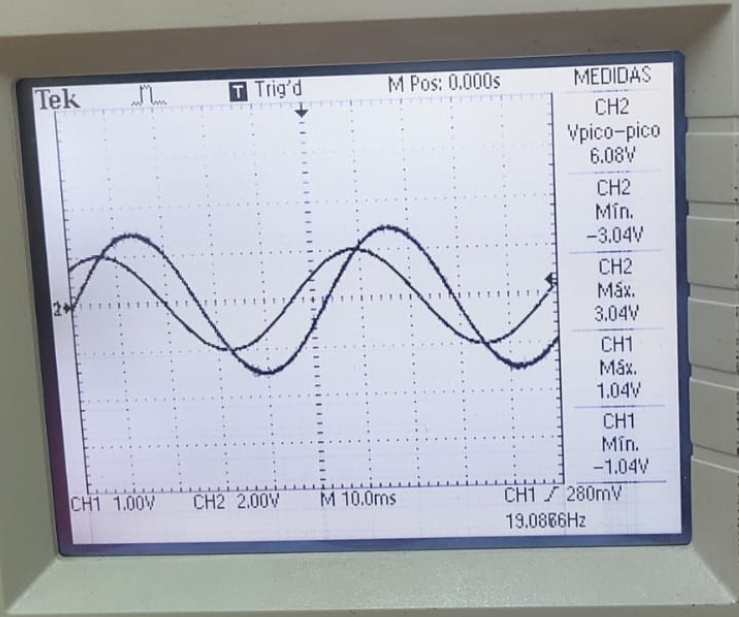
\includegraphics[width=\linewidth]{pot_max_f20hz_pto6.png}
        \caption{\(20\,\mathrm{Hz}\).}
    \end{subfigure}\hfill
    \begin{subfigure}[t]{0.48\textwidth}
        \centering
        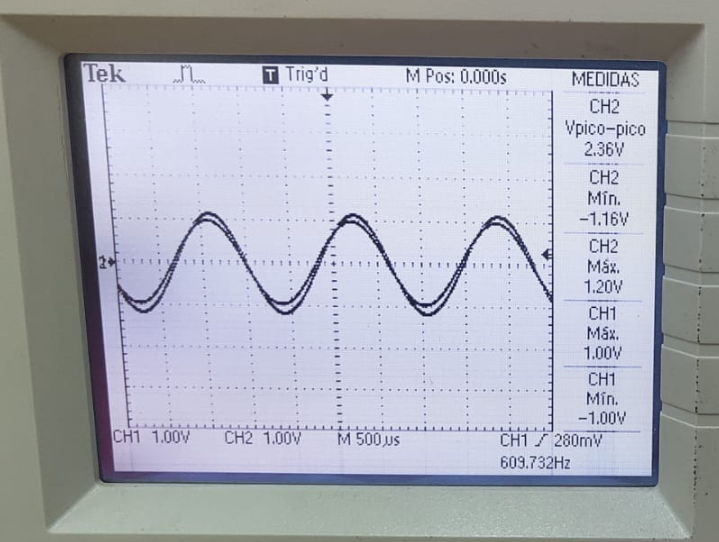
\includegraphics[width=\linewidth]{pot_max_f600hz_pto6.png}
        \caption{\(600\,\mathrm{Hz}\).}
    \end{subfigure}

    \vspace{0.7em}
    \begin{subfigure}[t]{0.48\textwidth}
        \centering
        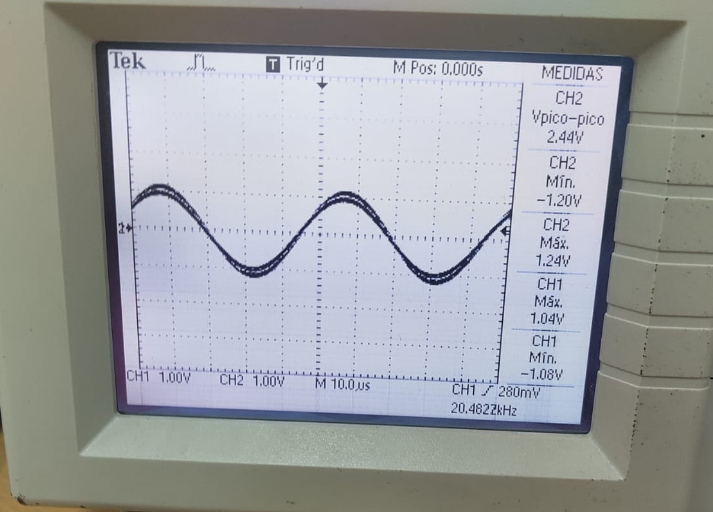
\includegraphics[width=\linewidth]{pot_max_f20khz_pto6.png}
        \caption{\(20\,\mathrm{kHz}\).}
    \end{subfigure}
    \caption{Capturas del osciloscopio con los potenciómetros al máximo.}
    \label{fig:max-scopes}
\end{figure}


\section{Potenciómetros al mínimo}

\measurementtable{
    \caption{Resultados con ambos potenciómetros al mínimo.}
    \label{tab:min}
    \begin{tabular}{>{\bfseries}c c c c c l}
        \toprule
        \(f\) & \(V_{i,pp}\) & \(V_{o,pp}\) & \(\lvert A_v\rvert\) & \(G\) & Fase observada \\
        & (V) & (V) & & (dB) & \\
        \midrule
        20 Hz  & 2,08 & 1,04 & 0,50 & -6,02  & Lectura limitada por ruido \\
        600 Hz & 2,20 & 1,76 & 0,80 & -1,94  & Desfase visible \\
        20 kHz & 2,00 & 0,40 & 0,20 & -13,98 & Lectura limitada por atenuación \\
        \bottomrule
    \end{tabular}
}

La salida queda atenuada en las tres frecuencias. A \(20\,\mathrm{Hz}\) el ruido sobre CH2
dificulta una lectura precisa del desplazamiento temporal; a \(600\,\mathrm{Hz}\) el desfase
es visible, y a \(20\,\mathrm{kHz}\) la fuerte atenuación vuelve poco confiable una
determinación cuantitativa de fase a partir de la captura.

\begin{figure}[H]
    \centering
    \begin{subfigure}[t]{0.48\textwidth}
        \centering
        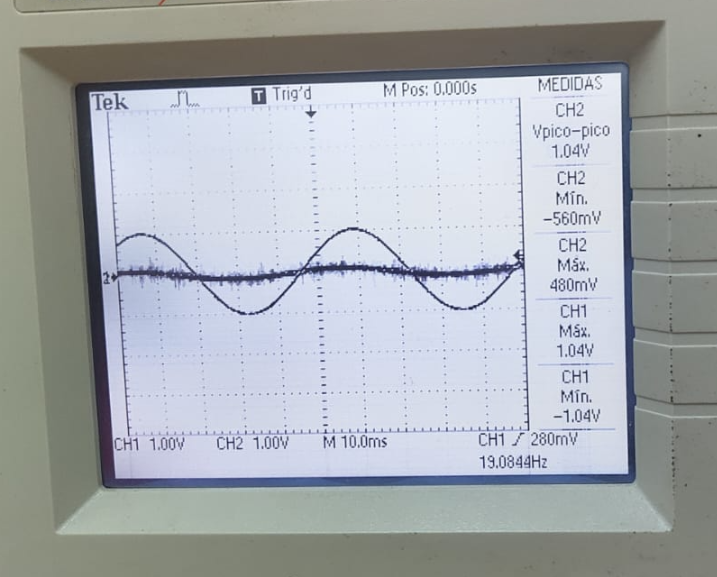
\includegraphics[width=\linewidth]{pot_min_f20hz_pto7.png}
        \caption{\(20\,\mathrm{Hz}\).}
    \end{subfigure}\hfill
    \begin{subfigure}[t]{0.48\textwidth}
        \centering
        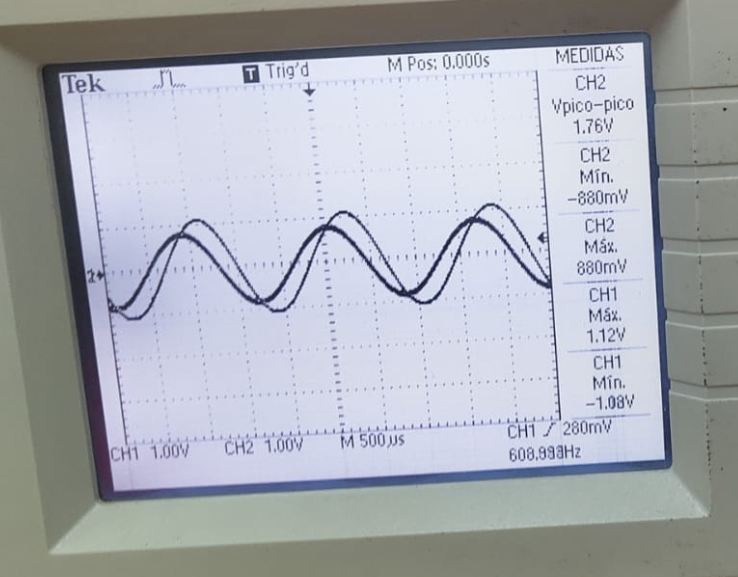
\includegraphics[width=\linewidth]{pot_min_f600hz_pto7.png}
        \caption{\(600\,\mathrm{Hz}\).}
    \end{subfigure}

    \vspace{0.7em}
    \begin{subfigure}[t]{0.48\textwidth}
        \centering
        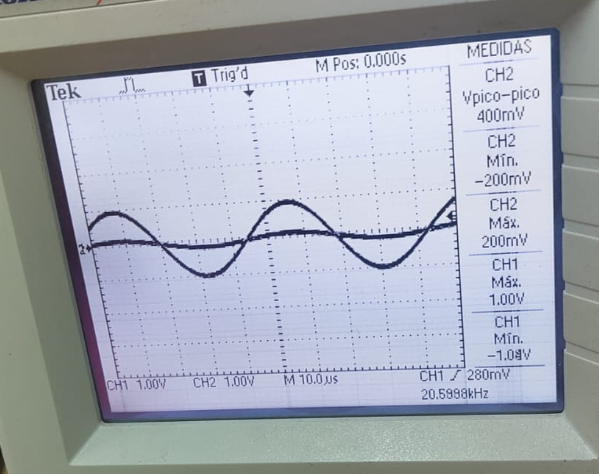
\includegraphics[width=\linewidth]{pot_min_f20khz_pto7.png}
        \caption{\(20\,\mathrm{kHz}\).}
    \end{subfigure}
    \caption{Capturas del osciloscopio con los potenciómetros al mínimo.}
    \label{fig:min-scopes}
\end{figure}

\section{Potenciómetros a mitad de recorrido}

\measurementtable{
    \caption{Resultados con ambos potenciómetros a mitad de recorrido.}
    \label{tab:mid}
    \begin{tabular}{>{\bfseries}c c c c c l}
        \toprule
        \(f\) & \(V_{i,pp}\) & \(V_{o,pp}\) & \(\lvert A_v\rvert\) & \(G\) \\
        & (V) & (V) & & (dB) & \\
        \midrule
        20 Hz  & 2,04 & 1,60 & 0,78 & -2,11 \\
        600 Hz & 2,00 & 1,44 & 0,72 & -2,85 \\
        20 kHz & 2,08 & 1,20 & 0,58 & -4,78 \\
        \bottomrule
    \end{tabular}
}

\begin{figure}[H]
    \centering
    \begin{subfigure}[t]{0.48\textwidth}
        \centering
        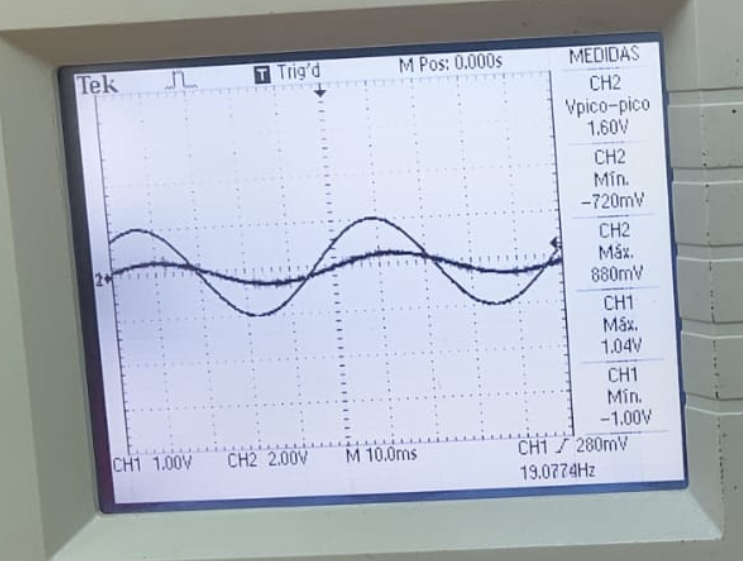
\includegraphics[width=\linewidth]{pot_mid_f20hz_pto8.png}
        \caption{\(20\,\mathrm{Hz}\).}
    \end{subfigure}\hfill
    \begin{subfigure}[t]{0.48\textwidth}
        \centering
        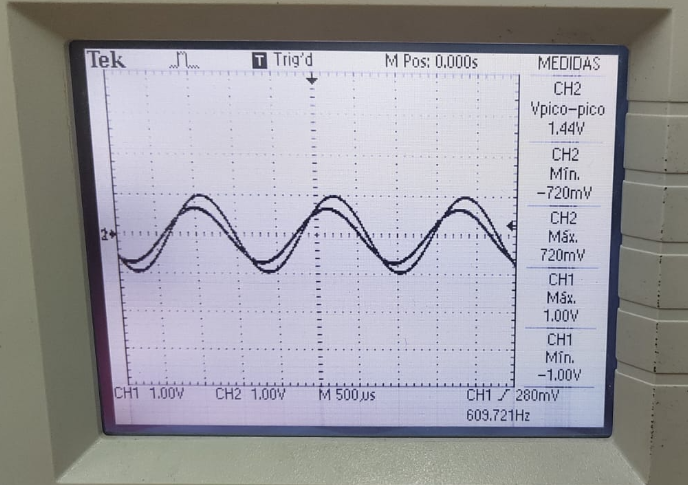
\includegraphics[width=\linewidth]{pot_mid_f600hz_pto8.png}
        \caption{\(600\,\mathrm{Hz}\).}
    \end{subfigure}

    \vspace{0.7em}
    \begin{subfigure}[t]{0.48\textwidth}
        \centering
        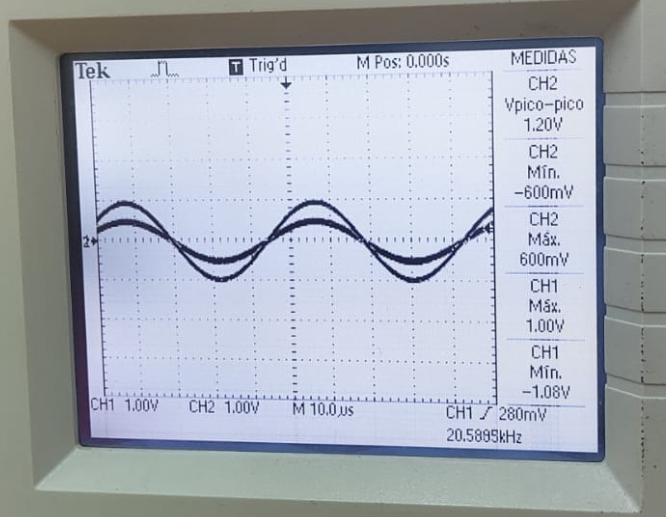
\includegraphics[width=\linewidth]{pot_mid_f20khz_pto8.png}
        \caption{\(20\,\mathrm{kHz}\).}
    \end{subfigure}
    \caption{Capturas del osciloscopio con los potenciómetros a mitad de recorrido.}
    \label{fig:mid-scopes}
\end{figure}

\section{Barrido en frecuencia}

\begin{figure}[H]
    \centering
    \begin{tikzpicture}
        \begin{axis}[
            width=0.96\textwidth,
            height=0.54\textwidth,
            xmode=log,
            log basis x=10,
            xmin=20,
            xmax=20000,
            ymin=-20,
            ymax=16,
            xlabel={Frecuencia (Hz)},
            ylabel={Ganancia (dB)},
            grid=both,
            minor grid style={gray!15},
            major grid style={gray!35},
            tick label style={font=\small},
            label style={font=\small},
            legend style={at={(0.5,-0.22)},anchor=north,legend columns=3,font=\small},
            line width=1pt,
            mark size=2pt
        ]
        \addplot[color=utnblue,mark=*] coordinates {
            (20,9.54) (50,4.17) (100,3.52) (200,1.80)
            (500,2.07) (1000,1.24) (2000,1.53) (5000,6.19)
            (10000,10.39) (12000,11.87) (15000,13.57) (20000,13.98)
        };
        \addlegendentry{Máximo}

        \addplot[color=black,mark=square*] coordinates {
            (20,-1.45) (50,-7.47) (100,-9.21) (200,-9.21)
            (500,-5.38) (1000,-3.19) (2000,-0.34) (5000,0)
            (10000,-0.33) (12000,-0.70) (15000,-0.67) (20000,-1.02)
        };
        \addlegendentry{Mitad}

        \addplot[color=alertred,mark=triangle*] coordinates {
            (20,-18.76) (50,-16.26) (100,-12.74) (200,-9.21)
            (500,-9.21) (1000,-11.40) (2000,-14.32) (5000,-16.26)
            (10000,-16.26) (12000,-16.26) (15000,-16.26) (20000,-16.26)
        };
        \addlegendentry{Mínimo}
        \end{axis}
    \end{tikzpicture}
    \caption{Respuesta en frecuencia obtenida de las tablas de medición.}
    \label{fig:sweep}
\end{figure}

\begin{table}[H]
    \centering
    \caption{Barrido con los potenciómetros al máximo.}
    \label{tab:sweep-max}
    \small
    \begin{tabular}{r r r r}
        \toprule
        \textbf{Frecuencia (Hz)} & \(V_o\) (V) & \(V_i\) (V) & \textbf{dB} \\
        \midrule
        20    & 3,12 & 1,04 & 9,54 \\
        50    & 1,68 & 1,04 & 4,17 \\
        100   & 1,56 & 1,04 & 3,52 \\
        200   & 1,28 & 1,04 & 1,80 \\
        500   & 1,32 & 1,04 & 2,07 \\
        1000  & 1,20 & 1,04 & 1,24 \\
        2000  & 1,24 & 1,04 & 1,53 \\
        5000  & 2,12 & 1,04 & 6,19 \\
        10000 & 3,44 & 1,04 & 10,39 \\
        12000 & 4,08 & 1,04 & 11,87 \\
        15000 & 4,96 & 1,04 & 13,57 \\
        20000 & 5,20 & 1,04 & 13,98 \\
        \bottomrule
    \end{tabular}
\end{table}

\clearpage
\begin{figure}[H]
    \centering
    \minsweepcapture{1}{20\,\mathrm{Hz}}\hfill
    \minsweepcapture{2}{50\,\mathrm{Hz}}

    \vspace{0.7em}
    \minsweepcapture{3}{100\,\mathrm{Hz}}\hfill
    \minsweepcapture{4}{200\,\mathrm{Hz}}

    \vspace{0.7em}
    \minsweepcapture{5}{500\,\mathrm{Hz}}\hfill
    \minsweepcapture{6}{1\,\mathrm{kHz}}
    \caption{Capturas del barrido máximo, mediciones 1 a 6.}
    \label{fig:sweep-max-1-6}
\end{figure}

\clearpage
\begin{figure}[H]
    \centering
    \minsweepcapture{7}{2\,\mathrm{kHz}}\hfill
    \minsweepcapture{8}{5\,\mathrm{kHz}}

    \vspace{0.7em}
    \minsweepcapture{9}{10\,\mathrm{kHz}}\hfill
    \minsweepcapture{10}{12\,\mathrm{kHz}}

    \vspace{0.7em}
    \minsweepcapture{11}{15\,\mathrm{kHz}}\hfill
    \minsweepcapture{12}{20\,\mathrm{kHz}}
    \caption{Capturas del barrido máximo, mediciones 7 a 12.}
    \label{fig:sweep-max-7-12}
\end{figure}

\clearpage
\begin{center}
    \begin{minipage}[t]{0.47\textwidth}
        \vspace{0pt}
        \centering
        \captionof{table}{Barrido con los potenciómetros al mínimo.}
        \label{tab:sweep-min}
        \footnotesize
        \begin{tabular}{r r r r}
            \toprule
            \textbf{Frecuencia (Hz)} & \(V_o\) (V) & \(V_i\) (V) & \textbf{dB} \\
            \midrule
            20    & 0,12 & 1,04 & -18,76 \\
            50    & 0,16 & 1,04 & -16,26 \\
            100   & 0,24 & 1,04 & -12,74 \\
            200   & 0,36 & 1,04 & -9,21 \\
            500   & 0,36 & 1,04 & -9,21 \\
            1000  & 0,28 & 1,04 & -11,40 \\
            2000  & 0,20 & 1,04 & -14,32 \\
            5000  & 0,16 & 1,04 & -16,26 \\
            10000 & 0,16 & 1,04 & -16,26 \\
            12000 & 0,16 & 1,04 & -16,26 \\
            15000 & 0,16 & 1,04 & -16,26 \\
            20000 & 0,16 & 1,04 & -16,26 \\
            \bottomrule
        \end{tabular}
    \end{minipage}
\end{center}

\begin{figure}[H]
    \centering
    \maxsweepcapture{1}{20\,\mathrm{Hz}}\hfill
    \maxsweepcapture{2}{50\,\mathrm{Hz}}

    \vspace{0.7em}
    \maxsweepcapture{3}{100\,\mathrm{Hz}}\hfill
    \maxsweepcapture{4}{200\,\mathrm{Hz}}

    \vspace{0.7em}
    \maxsweepcapture{5}{500\,\mathrm{Hz}}\hfill
    \maxsweepcapture{6}{1\,\mathrm{kHz}}
    \caption{Capturas del barrido mínimo, mediciones 1 a 6.}
    \label{fig:sweep-min-1-6}
\end{figure}

\clearpage
\begin{figure}[H]
    \centering
    \maxsweepcapture{7}{2\,\mathrm{kHz}}\hfill
    \maxsweepcapture{8}{5\,\mathrm{kHz}}

    \vspace{0.7em}
    \maxsweepcapture{9}{10\,\mathrm{kHz}}\hfill
    \maxsweepcapture{10}{12\,\mathrm{kHz}}

    \vspace{0.7em}
    \maxsweepcapture{11}{15\,\mathrm{kHz}}\hfill
    \maxsweepcapture{12}{20\,\mathrm{kHz}}
    \caption{Capturas del barrido mínimo, mediciones 7 a 12.}
    \label{fig:sweep-min-7-12}
\end{figure}
\clearpage
\begin{center}
    \begin{minipage}[t]{0.47\textwidth}
        \vspace{0pt}
        \centering
        \captionof{table}{Barrido con los potenciómetros a mitad de recorrido.}
        \label{tab:sweep-mid}
        \footnotesize
        \begin{tabular}{r r r r}
            \toprule
            \textbf{Frecuencia (Hz)} & \(V_o\) (V) & \(V_i\) (V) & \textbf{dB} \\
            \midrule
            20    & 0,88 & 1,04 & -1,45 \\
            50    & 0,44 & 1,04 & -7,47 \\
            100   & 0,36 & 1,04 & -9,21 \\
            200   & 0,36 & 1,04 & -9,21 \\
            500   & 0,56 & 1,04 & -5,38 \\
            1000  & 0,72 & 1,04 & -3,19 \\
            2000  & 1,00 & 1,04 & -0,34 \\
            5000  & 1,04 & 1,04 &     0 \\
            10000 & 1,04 & 1,08 & -0,33 \\
            12000 & 0,96 & 1,04 & -0,70 \\
            15000 & 1,00 & 1,08 & -0,67 \\
            20000 & 0,96 & 1,08 & -1,02 \\
            \bottomrule
        \end{tabular}
    \end{minipage}\hfill
\end{center}

\clearpage
\begin{figure}[H]
    \centering
    \midsweepcapture{1}{20\,\mathrm{Hz}}\hfill
    \midsweepcapture{2}{50\,\mathrm{Hz}}

    \vspace{0.7em}
    \midsweepcapture{3}{100\,\mathrm{Hz}}\hfill
    \midsweepcapture{4}{200\,\mathrm{Hz}}

    \vspace{0.7em}
    \midsweepcapture{5}{500\,\mathrm{Hz}}\hfill
    \midsweepcapture{6}{1\,\mathrm{kHz}}
    \caption{Capturas del barrido medio, mediciones 1 a 6.}
    \label{fig:sweep-mid-1-6}
\end{figure}

\clearpage
\begin{figure}[H]
    \centering
    \midsweepcapture{7}{2\,\mathrm{kHz}}\hfill
    \midsweepcapture{8}{5\,\mathrm{kHz}}

    \vspace{0.7em}
    \midsweepcapture{9}{10\,\mathrm{kHz}}\hfill
    \midsweepcapture{10}{12\,\mathrm{kHz}}

    \vspace{0.7em}
    \midsweepcapture{11}{15\,\mathrm{kHz}}\hfill
    \midsweepcapture{12}{20\,\mathrm{kHz}}
    \caption{Capturas del barrido medio, mediciones 7 a 12.}
    \label{fig:sweep-mid-7-12}
\end{figure}

\clearpage

La respuesta medida cubre desde \(-18{,}76\,\mathrm{dB}\) hasta
\(13{,}98\,\mathrm{dB}\). En la posición máxima se obtiene realce en ambos
extremos de la banda; en la posición media la respuesta se aproxima a \(0\,\mathrm{dB}\) por
encima de \(2\,\mathrm{kHz}\), mientras que la posición mínima presenta atenuación en todo
el barrido.

\section{Medición de Slew Rate}

El Slew Rate de la primera etapa se determina aplicando una señal cuadrada de amplitud y
frecuencia suficientes para que la pendiente de salida quede limitada por el operacional. Sobre
el flanco lineal se mide \(\Delta V\) y \(\Delta t\), y se calcula:
\[
    SR=\frac{\Delta V_o}{\Delta t}
\]

En la captura se obtiene \(\Delta t=680\,\mathrm{ns}=0{,}68\,\mathrm{\mu s}\) para una
variación aproximada de \(\Delta V=1{,}00\,\mathrm{V}\). Por lo tanto, el valor medido es:
\[
    SR=\frac{\Delta V}{\Delta t}
      =\frac{1{,}00\,\mathrm{V}}{0{,}68\,\mathrm{\mu s}}
      =\boxed{1{,}47\,\mathrm{V/\mu s}}.
\]

\begin{figure}[H]
    \centering
    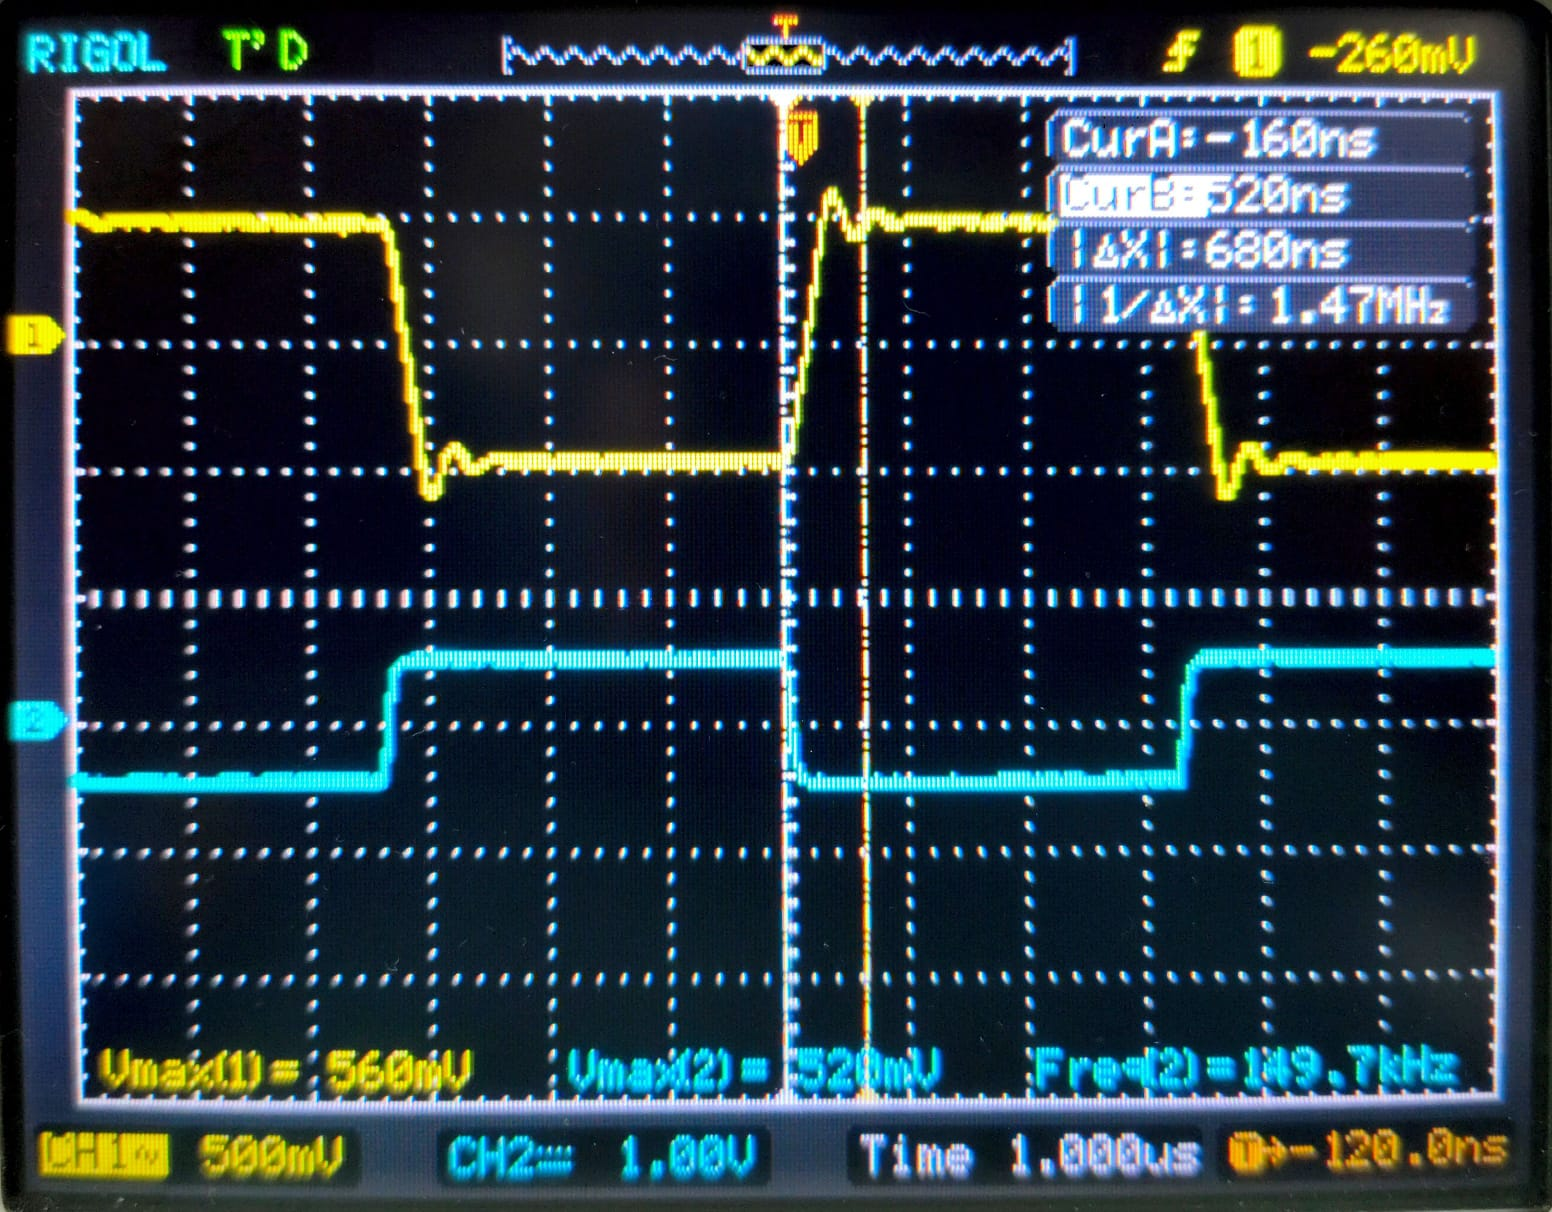
\includegraphics[width=0.88\textwidth]{Slew_Rate.jpg}
    \caption{Medición del Slew Rate de la primera etapa.}
    \label{fig:slew-rate}
\end{figure}

Esto coincide con el valor indicado en el datasheet de Texas Instruments correspondiente
al amplificador operacional RC4558, en el cual el valor mínimo es $\mathrm{1.1\ V /\mu s}$
y el típico $\mathrm{2.2\ V /\mu s}$

\section{Vistas del PCB en el software de diseño}

\begin{figure}[H]
    \centering
    \begin{subfigure}[t]{0.48\textwidth}
        \centering
        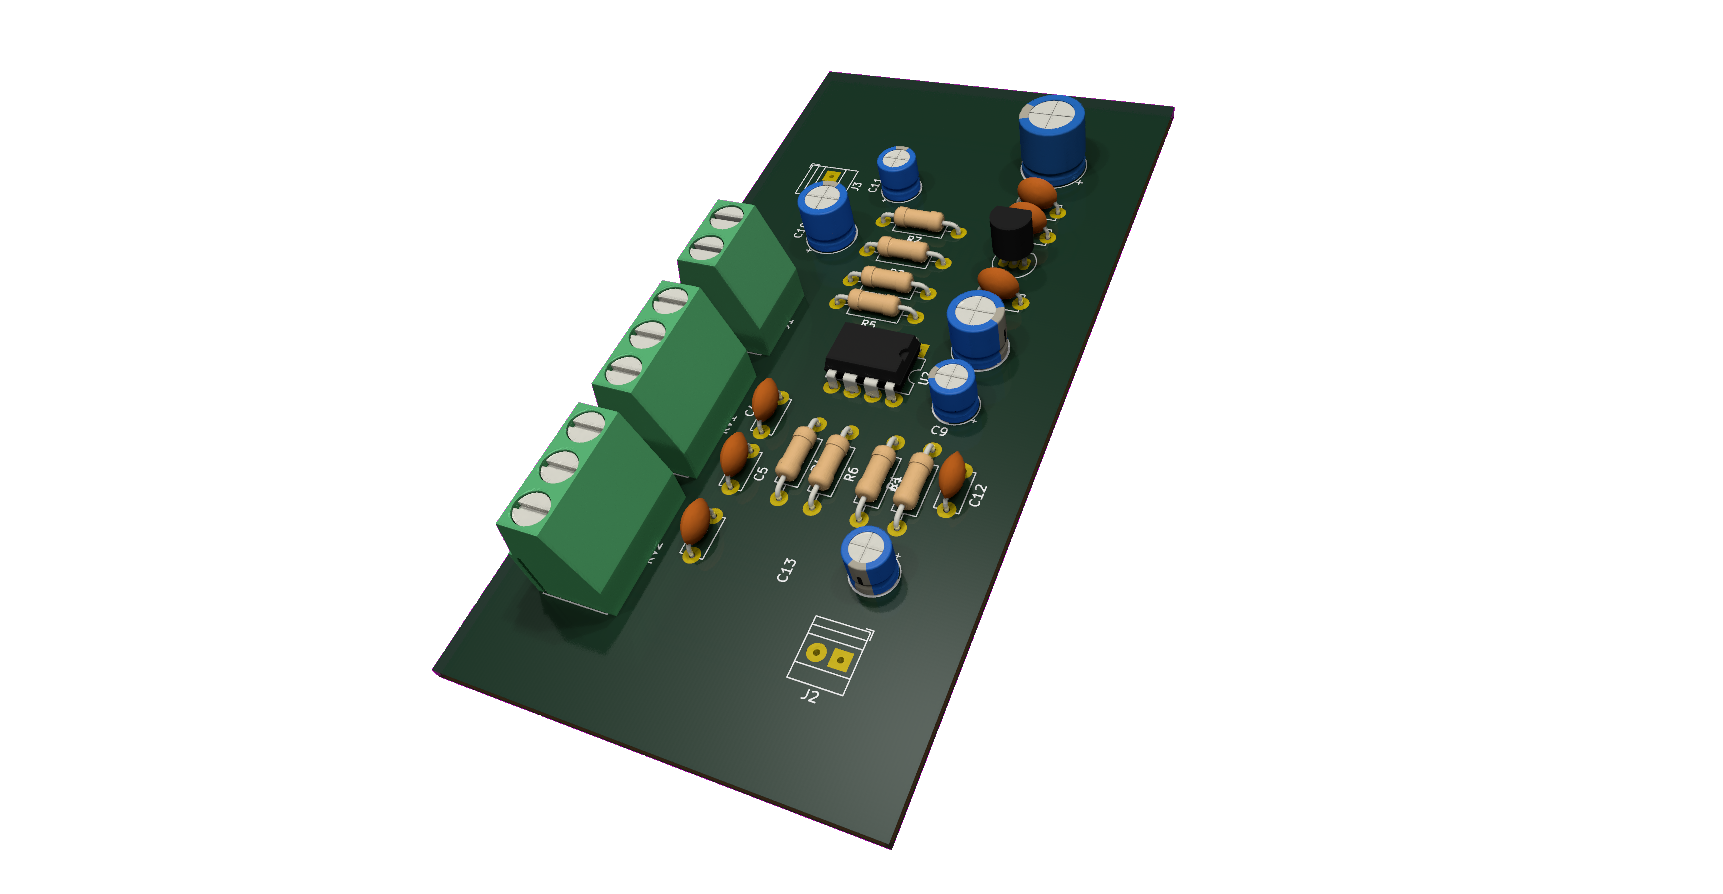
\includegraphics[trim=250 30 250 30,clip,width=\linewidth]{PCB_Front.png}
        \caption{Vista superior del PCB.}
        \label{fig:pcb-front}
    \end{subfigure}\hfill
    \begin{subfigure}[t]{0.48\textwidth}
        \centering
        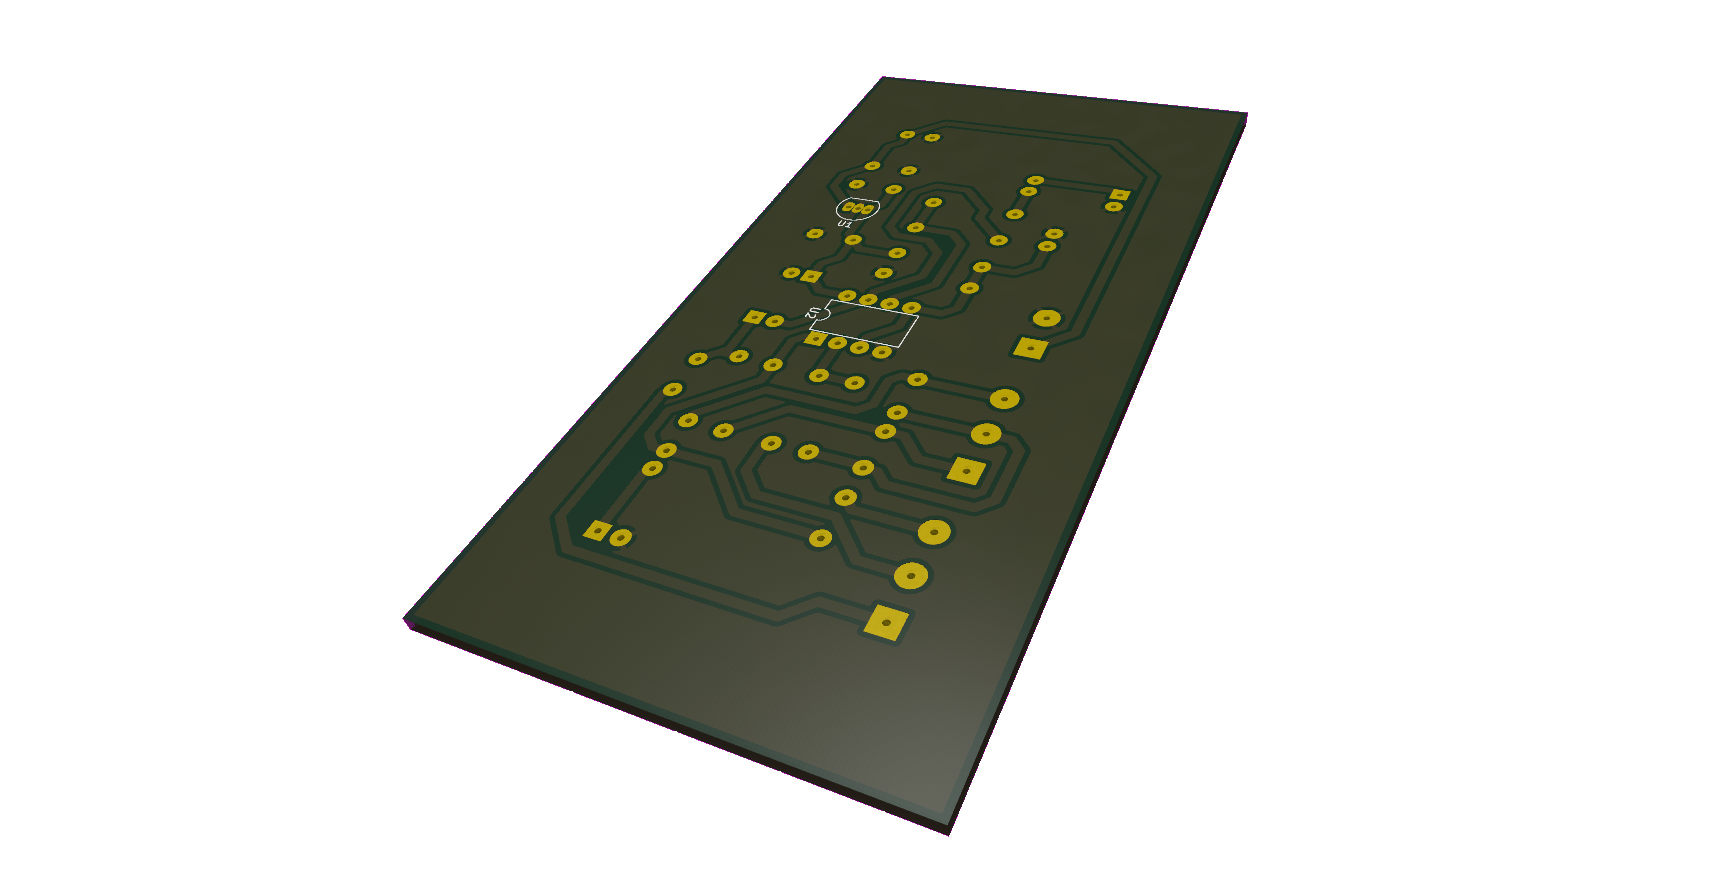
\includegraphics[trim=250 30 250 30,clip,width=\linewidth]{PCB_Rear.png}
        \caption{Vista inferior del PCB.}
        \label{fig:pcb-rear}
    \end{subfigure}
    \caption{Vistas del modelo 3D del PCB generadas en KiCad.}
    \label{fig:pcb-3d}
\end{figure}

\section{Fotografías de la placa armada}

\begin{figure}[H]
    \centering
    \begin{subfigure}[t]{0.27\textwidth}
        \centering
        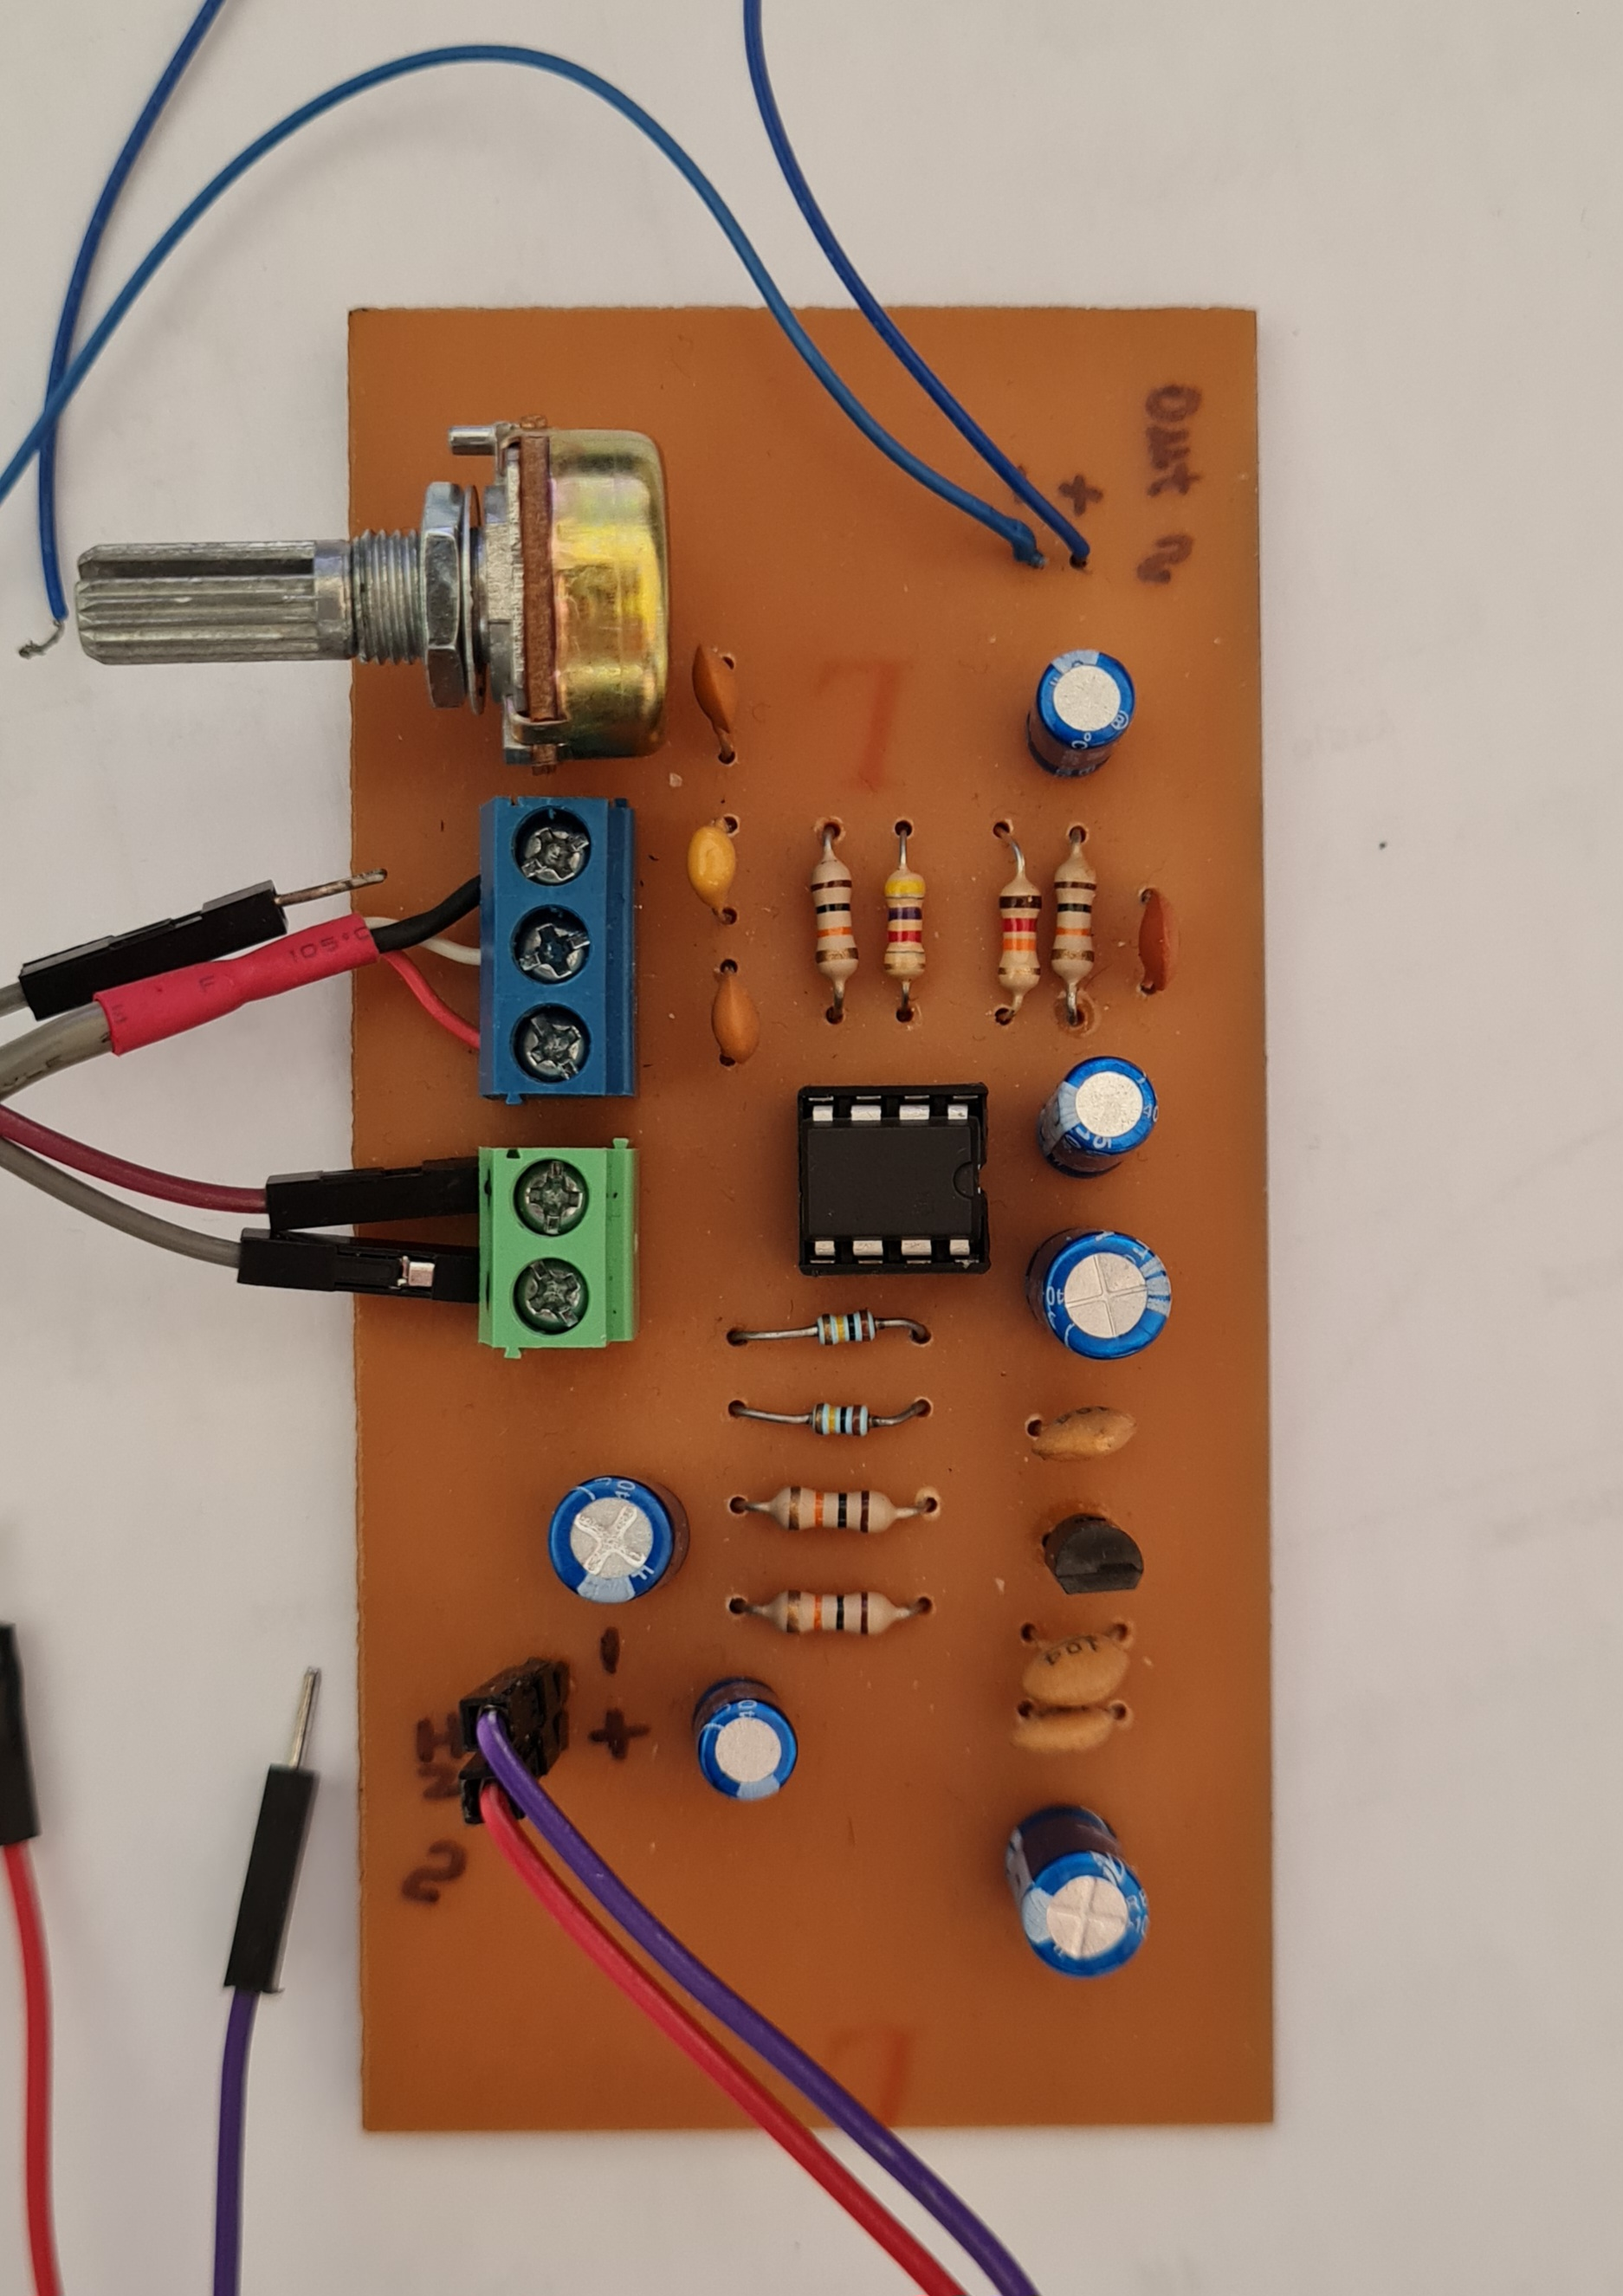
\includegraphics[width=\linewidth]{PCB_Front_Real.jpg}
        \caption{Cara de componentes.}
    \end{subfigure}\hspace{0.25\textwidth}
    \begin{subfigure}[t]{0.27\textwidth}
        \centering
        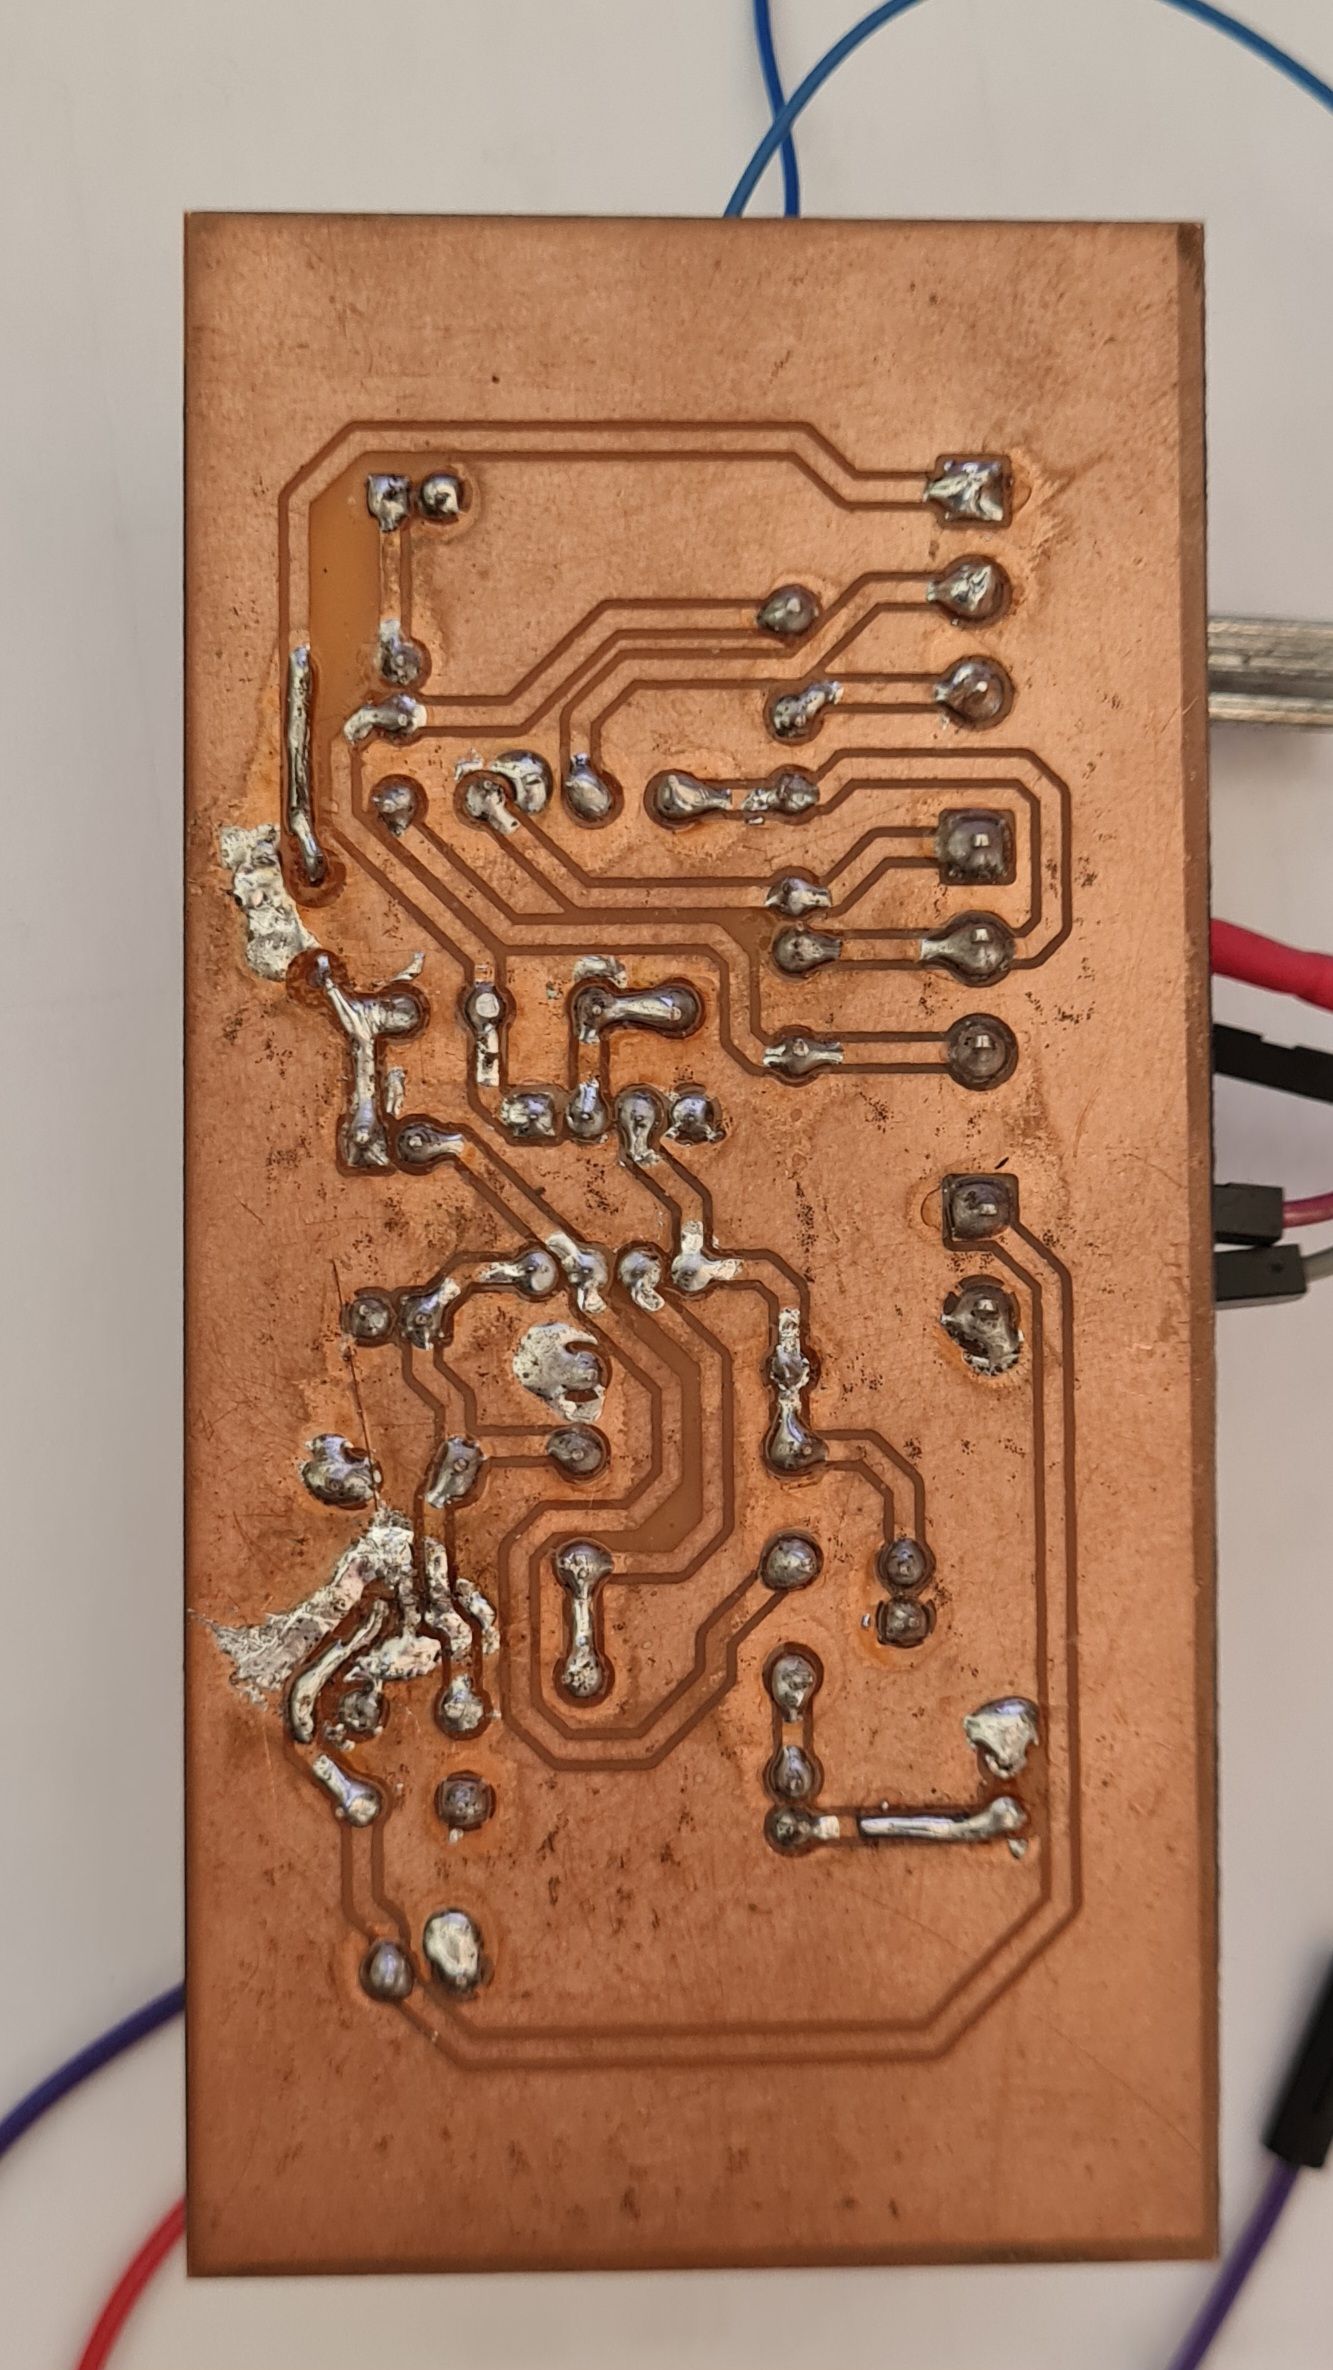
\includegraphics[width=\linewidth]{PCB_Rear_Real.jpg}
        \caption{Cara de cobre y soldaduras.}
    \end{subfigure}
    \caption{PCB construido. Difiere respecto a la figura \ref{fig:pcb-front} debido a que
    fue necesario que el potenciómetro RV2, correspondiente a las frecuencias altas, se
encuentre soldado en la placa para que la manipulación del mismo introduzca el menor ruido
posible en la señal de salida.}
    \label{fig:real-pcb}
\end{figure}

\section*{Conclusiones}
\addcontentsline{toc}{section}{Conclusiones}

El circuito implementa un control Baxandall con fuente simple mediante una referencia interna
de \(6\,\mathrm{V}\) y acoplamientos que bloquean la continua en entrada y salida. Las
capturas de los puntos 6 a 8 muestran cambios de amplitud y fase al variar la posición de los
potenciómetros. El barrido tabulado confirma una variación total entre
\(-18{,}76\,\mathrm{dB}\) y \(13{,}98\,\mathrm{dB}\) dentro de la banda de audio. El
Slew Rate medido en la primera etapa fue de \(1{,}47\,\mathrm{V/\mu s}\).

Para cerrar la documentación experimental sin introducir datos no medidos, quedan por agregar
la evidencia de simulación solicitada y la excursión máxima. También debe
confirmarse el criterio dimensional aplicado al PCB de \(100\,\mathrm{mm}\times 50\,\mathrm{mm}\).

\end{document}
